%%%%%%%%%%%%%%%%%%%%%%%%%%%%%%%%%%%%%%%%%%%%%%%%%%%%%%%%%%%%%%%%%%%%
%% I, the copyright holder of this work, release this work into the
%% public domain. This applies worldwide. In some countries this may
%% not be legally possible; if so: I grant anyone the right to use
%% this work for any purpose, without any conditions, unless such
%% conditions are required by law.
%%%%%%%%%%%%%%%%%%%%%%%%%%%%%%%%%%%%%%%%%%%%%%%%%%%%%%%%%%%%%%%%%%%%

% This theme was based on fibeamer theme 
% If you found any bugs please contact @karlosos
% This repository is hosted on github https://github.com/karlosos/zut-fibeamer/

\documentclass{beamer}
\usetheme[faculty=wi]{fibeamer}
\usepackage[utf8]{inputenc}
\usepackage[
  main=polish,
  polish
]{babel}

\title{Aula 8  - Banco de dados}
\subtitle{Tópicos especiais em Sistemas}
\author{Prof. Juliana Costa Silva}

\usepackage{ragged2e}  % `\justifying` text
\usepackage{booktabs}  % Tables
\usepackage{tabularx}
\usepackage{tikz}      % Diagrams
\usetikzlibrary{calc, shapes, backgrounds}
\usepackage{amsmath, amssymb}
\usepackage{url}       % `\url`s
\usepackage{listings}  % Code listings
\frenchspacing
\begin{document}

%------------------------------------------------------------------------
  \frame[c]{\maketitle}
      \begin{frame}<beamer>
      \frametitle{O que veremos hoje}
      \tableofcontents
    \end{frame}
%------------------------------------------------------------------------
%------------------------------------------------------------------------
    \section{Revendo...}
    \begin{frame}{Revendo...}{O que já aprendemos?}
      
      \begin{itemize}
            \item Criamos um projeto node;
            \item organizamos os arquivos de configuração na pasta config;
            \item Organizamos os controladores na pasta controllers;
            \item Configuramos ações de GET e POST para a rota \alert{movimento}.
            \item Enviamos dados em formato JSON
       \end{itemize}
       
     \end{frame}
     %------------------------------------------------------------------------
\begin{frame}[label=proof]{O projeto da disciplina}
	\begin{itemize}
	\item Faremos um sistema de controle financeiro pessoal;
	\item Este sistema deve ter:
	\begin{itemize}
	\item Registro de gastos;
	\item Login de usuários;
	\item Registro de renda (salários - comissões - negócios);
	\item Registro de cartões de créditos;
	\item Registro de contas bancárias;
	\end{itemize}
	\end{itemize}
    \end{frame}
%------------------------------------------------------------------------
    \begin{frame}[label=lists]{Utilizaremos MySQL}
      \begin{columns}[onlytextwidth]
        \column{.5\textwidth}
          \begin{itemize}
            \item Para utilizarmos o MySQL instalaremos o package;
            \item No terminal digite \alert{npm install mysql}
            \item No MySQL crie um banco de dados chamado  \textbf{wallet}; 
          \end{itemize}
        \column{.5\textwidth}
            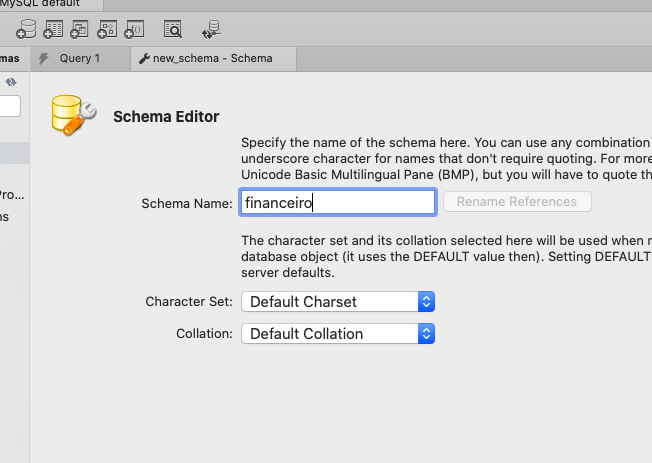
\includegraphics[width=65mm]{resources/aula6_1.png}
      \end{columns}
    \end{frame}

%------------------------------------------------------------------------
\section{Infraestrutura}
    \begin{frame}[label=lists]{Infraestrutura}
    \begin{exampleblock}{Pasta de infraestrutura}
        	\begin{itemize}
	\item Essa pasta será responsável por arquivos de infraestrutura;
	\item Tudo o que é necessário para a aplicação funcionar além das regras de negócio;
	\item Crie uma pasta \alert{infra} e dentro dela o arquivo \textbf{conncetion.js}.
        	\end{itemize}
      \end{exampleblock}
      \tiny{\textbf{Fonte:} \cite{nodejs2022api}}
    \end{frame}
%------------------------------------------------------------------------
\section{Conexão}
    \begin{frame}[label=lists]{Conexão}

% \begin{columns}[onlytextwidth]
%        \column{.5\textwidth}
         Para realizar a conexãoimportaremos o pacote \textbf{mysql}
         \begin{itemize}
         \item No arquivo \textbf{connection.js};
         \item Vamos acrescentar o código com os dados da nossa conexão;
         \end{itemize}
%        \column{.5\textwidth}
	            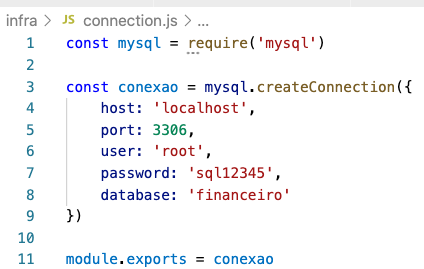
\includegraphics[width=80mm]{resources/aula6_3.png}\\
            \tiny{\textbf{Fonte:} O autor}
%      \end{columns}
        \tiny{\textbf{Fonte:} \cite{moziladev2022}}
    \end{frame}

 %------------------------------------------------------------------------
    \begin{frame}[label=lists]{Problemas}
    No Terminal, notaremos que que rodamos o servidor antes mesmo da mensagem do sucesso da conexão, então executou independentemente.
   \begin{itemize}
       \item Se a conexão não der certo a aplicação não deveria funcionar;
       \item Devemos iniciar a aplicação com a conexão ao banco de dados e após ela iniciar o app.
       \item Para isso acrescentaremos o \alert{else} na inicialização;
    \end{itemize}
    \end{frame}
     %------------------------------------------------------------------------
    \begin{frame}[label=lists]{Else}
    No \alert{else} colocaremos a inicialização da aplicação, que só ocorrerá se \alert{erro} for falso;
	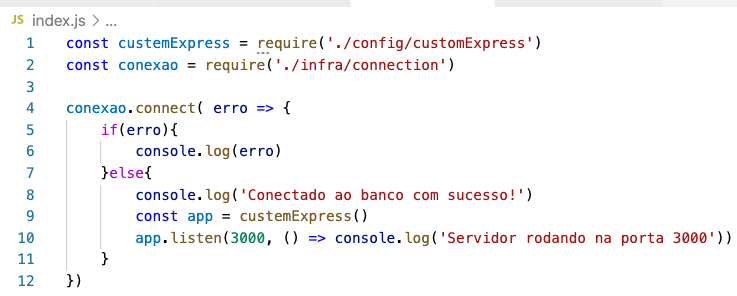
\includegraphics[width=110mm]{resources/aula6_4.png}\\
            \tiny{\textbf{Fonte:} O autor}

    \end{frame}
   
 %------------------------------------------------------------------------
 \section{Criando tabelas}
    \begin{frame}[label=lists]{tabelas.js}
    Criaremos um arquivo \textbf{tabelas.js}, na pasta infra.
	\begin{exampleblock}{Editando tabelas.js}
		\begin{itemize}
			\item Nesse arquivo criaremos a classe \alert{Tabelas};
			\item Esta classe será responsável por criar tabelas no banco de dados;
			\item Dentro da classe \alert{Tabelas} neste arquivo, aplicaremos o método \alert{init()} 
			\item O método init() iniciará nosso trabalho;
			\item Receberemos a \alert{conexao} do banco de dados por parâmetro, que o deixará desacoplado sem que saiba de onde vem exatamente.
			\item Nesta conexão, escreveremos no \alert{console.log()} para identificar se realmente a class está sendo chamada.
		\end{itemize}
	\end{exampleblock}
	     \end{frame}
   
    %------------------------------------------------------------------------
    \begin{frame}[label=lists]{tabelas.js}
	\begin{center}
    		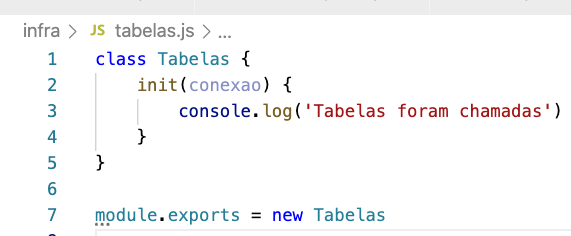
\includegraphics[width=110mm]{resources/aula6_5.png}\\
	        \tiny{ Código no arquivo \textbf{tabelas.js}. \textbf{Fonte:} O autor}
	 \end{center}
    \end{frame}
 %------------------------------------------------------------------------
    \begin{frame}[label=proof]{Teste Tabelas}
    \begin{alertblock}{index.js}
	\begin{itemize}
	\item Já dentro de \textbf{index.js}, quando conectarmos com o banco, queremos que este conecte e já crie as tabelas que precisamos.
	\item Neste arquivo, importaremos Tabelas sendo igual a \alert{require()} recebendo o caminho do \textbf{tabela.js}.
	\item Executaremos a importação e, antes de criarmos app igual a \alert{customExpress()}, teremos Tabelas com \alert{.init()} recebendo a \alert{conexao} que estamos usando, importada da infraestrutura.
	\end{itemize}
	\end{alertblock}
    \end{frame}
 %------------------------------------------------------------------------
    \begin{frame}{index.js}
         \begin{center}
    	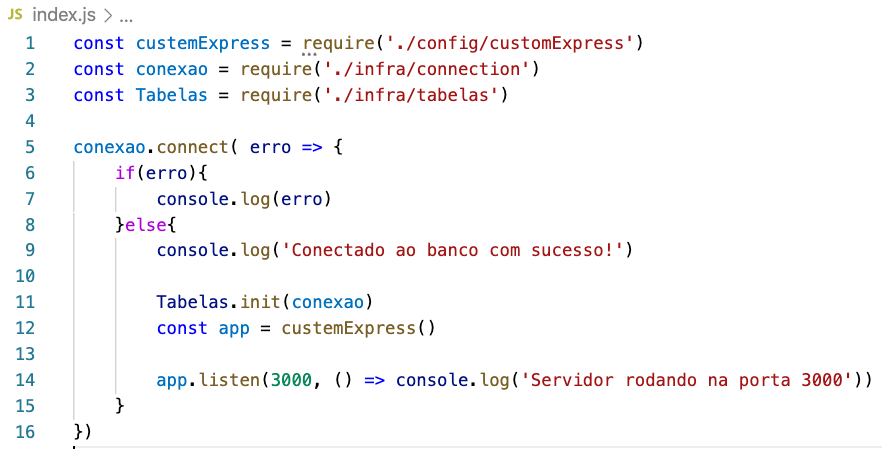
\includegraphics[width=110mm]{resources/aula6_6.png}\\
        \tiny{ Código no arquivo \textbf{index.js}. \textbf{Fonte:} O autor}
     \end{center}   
    \end{frame}
  %-----------------------------------------------------------------------------
  \begin{frame}{Método criarMovimento}
   \begin{itemize}
   \item Agora poderemos criar as tabelas; 
   \item No arquivo \textbf{tabelas.js}, geraremos um novo método chamado \alert{criarMovimentos()} e usaremos esta conexao;
   \item Para conectarmos, precisaremos passar para nosso escopo com \alert{this} no lugar de \alert{console.log()};
   \item Então dentro do método, digitaremos this com .conexao chamando uma .query() que espera uma query SQL para podermos executar, e logo em seguida espera também uma função a ser executada na sequência.
   \end{itemize}
  \end{frame}
  %------------------------------------------------------------------------
    \begin{frame}{tabelas.js}
         \begin{center}
    	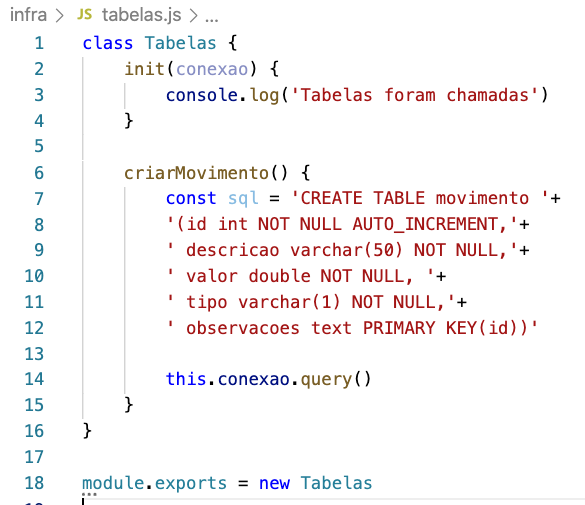
\includegraphics[width=85mm]{resources/aula6_7.png}\\
        \tiny{ Código no arquivo \textbf{tabelas.js}. \textbf{Fonte:} O autor}
     \end{center}   
    \end{frame}
    %-----------------------------------------------------------------------------
  \begin{frame}{Ainda sobre o Método criarMovimento}
  Ainda não estamos executando a \alert{query()}
   \begin{itemize}
   \item Após \alert{const sql}, passaremos a função que será executada quando a tabela for criada. 
   \item O primeiro parâmetro que receberá será o erro.
   \item Logo, se a \alert{query()} não for executada, o sistema indicará algum erro. 
   \item Portanto, \alert{if()} recebendo o erro imprimirá a falha. Caso contrário, imprimirá a \textcolor{blue}{Tabela Movimentos criada com sucesso}.
   \item O \alert{init()} deverá chamar a tabela, e este método por sua vez está sendo chamado dentro do \textbf{index.js}. 
   \item Logo, digitaremos this com \alert{.criarMovimentos()}.
   \end{itemize}
  \end{frame}
  
  %------------------------------------------------------------------------
    \begin{frame}{tabelas.js}
         \begin{center}
    	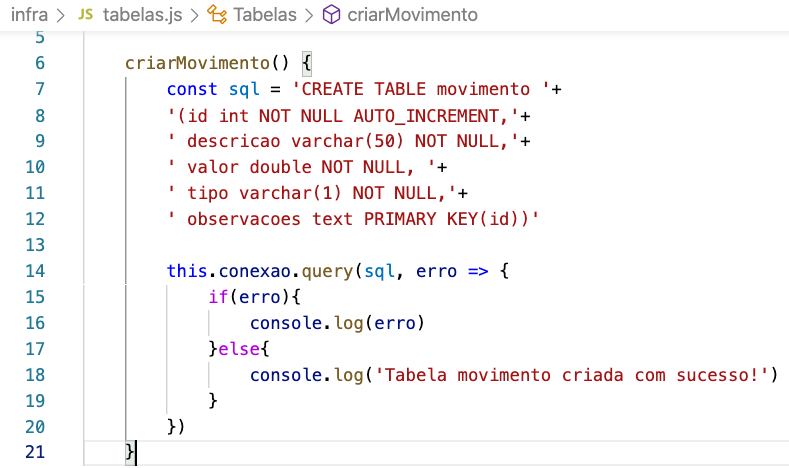
\includegraphics[width=100mm]{resources/aula6_8.png}\\
        \tiny{ Código no arquivo \textbf{tabelas.js}. \textbf{Fonte:} O autor}
     \end{center}   
    \end{frame}

  %------------------------------------------------------------------------
    \begin{frame}{tabelas.js chamando o método no init()}
         \begin{center}
    	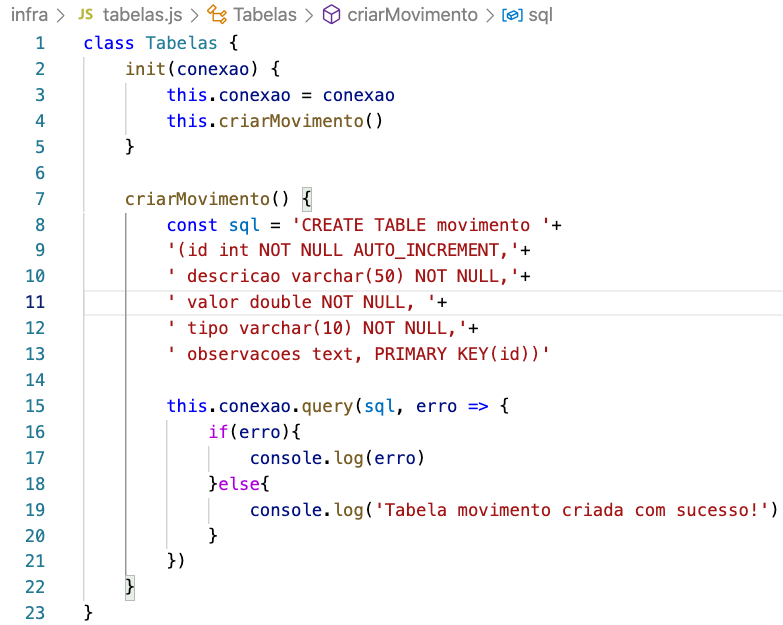
\includegraphics[width=100mm]{resources/aula6_9.png}\\
        \tiny{ Código no arquivo \textbf{tabelas.js}. \textbf{Fonte:} O autor}
     \end{center}   
    \end{frame}

%------------------------------------------------------------------------
 %-----------------------------------------------------------------------------
  \section{Atividade}
  \begin{frame}{Atividade de aula}
   \begin{enumerate}
     \item Desenvolva a rota \textbf{carteiras};
     \item Essa rota cuidará do cadastro de diferentes carteiras no orçamento pessoal;
     \item Desenvolva o GET  e POST dessa rota, e identifique os dados em formato JSON para cadastrar uma carteira; 
     \item Envie como respostas o código de carteira.js e o JSON enviado via Postman nos testes (impresso no console).
   \end{enumerate}
  \end{frame}
%------------------------------------------------------------

%------------------------------------------------------------------------
\section{Referências}
\begin{frame}{Referências}%[allowframebreaks]
\small
\begin{center}
\tiny
\bibliographystyle{apalike}
\bibliography{ref_aula}
\end{center}
\end{frame}
  
\end{document}